\chapter{Analyses}\label{ch:Analysis}
In this chapter, an analysis of the data collected via the methods described in
the previous chapter (\autoref{ch:Methods}) is given. Firstly, a brief
initial overview is provided, where descriptive statistics of the equilibria
obtained and the overall characteristics of the strategies used are discussed.
Following this, a critical analysis of the \(p\)-thresholds obtained is carried
out. Here, the environmental effects, on the outcome of the game, discussed
include: number of opponents and level of added noise. Note, the final database
has
\input{src/database_code/data/se/20_01_2020/entries-in-database.txt} entries (rows) and a total number of 
\input{src/database_code/data/se/20_01_2020/number-of-tournaments.txt} player
sets. This dataset has been archived at ().

Before this, a reminder that any analysis stated, in this chapter, on degeneracy
is purely from those identified by Nashpy. This implies that there may be
further degeneracy that was unidentified.

\section{Initial Analysis}\label{sec:Initial_Analysis}
In this section, all the games (including those identified as degenerate)
are considered. Taking a brief look at the graphs produced for each set of
tournaments, it can be seen that the main `shapes' obtained are as seen in~\autoref{fig:example_graphs}.

\begin{figure}
    \begin{subfigure}{0.45\textwidth}
        \centering
        \includegraphics[width=\textwidth]{folk_thm/single_game/2/0/0.0/main.pdf}
        \caption{2-player tournament set with \(p_{n}=0\), one stochastic player and no degeneracy identified.}\label{subfig:clear_thresh_plot}
    \end{subfigure}
    \begin{subfigure}{0.45\textwidth}
        \centering
        \includegraphics[width=\textwidth]{folk_thm/single_game/6/110/0.0/main.pdf}
        \caption{6-player tournament set with \(p_{n}=0\), three stochastic players and potential degeneracy was yielded from 10 of the tournaments.}\label{subfig:unclear_thresh_plot}
    \end{subfigure}

    \begin{subfigure}{0.45\textwidth}
        \centering
        \includegraphics[width=\textwidth]{folk_thm/single_game/5/77/0.0/main.pdf}
        \caption{5-player tournament set with \(p_{n}=0\), two stochastic players and five tournaments played yielded potentially degenerate games.}\label{subfig:degenerate_plot}
    \end{subfigure}
    \begin{subfigure}{0.45\textwidth}
        \centering
        \includegraphics[width=\textwidth]{folk_thm/single_game/4/60/0.0/main.pdf}
        \caption{4-player game with \(p_{n}=0\), one stochastic player and no degeneracy identified.}\label{subfig:constant_plot}
    \end{subfigure}
    \caption{Example graphs obtained from the experiment.}\label{fig:example_graphs}
\end{figure}

In~\autoref{subfig:clear_thresh_plot}, a clear \(p\)-threshold of approximately
0.28 is apparent, clearly visualising the Folk Theorem. In this tournament set
the opponent was \textit{Inverse}, a stochastic player, indicating that perhaps
the stochasticity of a player does not affect the accuracy of the \(p\)-threshold. In~\autoref{subfig:unclear_thresh_plot}, the precise value of
the \(p\)-threshold is less clear, lying approximately in the range (0.1, 0.3). This
could be due to the potential degeneracy identified or just an element of
numerical experiment noise,
that appears within each tournament, possibly magnified by the number
of stochastic players. The opponents within this set
were: \textit{Feld: 1.0, 0.5, 200}; \textit{Cooperator};
\textit{EvolvedLookerUp2\_2\_2}; \textit{Tullock: 11}; and \textit{ZD-GEN-2:
0.125, 0.5, 3}\footnote{Note, these are the names of the strategies as
implemented in the Axelrod library and hence includes their corresponding parameters.}. \autoref{subfig:degenerate_plot} shows a potential problem
with the visualisation of the Folk Theorem when degenerate games are involved.
It becomes unclear as to what is happening in the graph,
especially regarding where the \(p\)-threshold lies. The opponents, in this case, were:
\textit{Random: 0.5}; \textit{Grumpy: Nice, 10, -10}; \textit{Fortress3}; and
\textit{Negation}. Finally,~\autoref{subfig:constant_plot} gives an example
of a tournament set for which there was always a non-zero probability of
defection, regardless of the \(p_{e}\) value. In this case, the
precision of game-ending probabilities chosen was not accurate enough to
identify the \(p\)-threshold. It implies that the tournament has to have an
ending probability of almost zero, within the interval (0, 0.001), in order for a
zero probability of defection to be rational. Here, the opponents of the
\textit{Defector} were: \textit{AntiCycler}; \textit{\(e\)}; and
\textit{Stalker: (D,)}. Similarly, it is observed that some graphs obtained
are constant at zero. Again this indicates that the precision of game-ending
probabilities was not fine enough to highlight the \(p\)-threshold. The ending probability of these tournaments has to lie within the interval
(0.999, 1). That is, almost immediately, the decision to defect is no longer
rational. Further research into these tournaments is highly recommended.

%\scalebox{0.52}{
%    \begin{table}
\centering
\caption{A table of the summary statistics produced from the data of the experiment.}
\label{tab:summary_stats}
\begin{tabular}{lrrrrrr}
\toprule
{} &  experiment\_number &  number\_of\_players &  tournament\_player\_set &  num\_of\_equilibria &  least\_prob\_of\_defection &  greatest\_prob\_of\_defection \\
\midrule
mean &      107364.481228 &           5.435509 &              97.105850 &           1.913727 &                 0.342275 &                    0.459722 \\
std  &       46880.538807 &           1.726832 &              42.619612 &           2.022014 &                 0.469061 &                    0.489564 \\
min  &           0.000000 &           2.000000 &               0.000000 &           1.000000 &                 0.000000 &                    0.000000 \\
25\%  &       72231.000000 &           4.000000 &              65.000000 &           1.000000 &                 0.000000 &                    0.000000 \\
50\%  &      114641.000000 &           6.000000 &             104.000000 &           1.000000 &                 0.000000 &                    0.000000 \\
75\%  &      147396.000000 &           7.000000 &             133.000000 &           3.000000 &                 1.000000 &                    1.000000 \\
max  &      175399.000000 &           8.000000 &             159.000000 &          39.000000 &                 1.000000 &                    1.000000 \\
\bottomrule
\end{tabular}
\end{table}

%}

The summary statistics are given in \autoref{tab:summary_stats}. From this, it can be
seen that the number of opponents the \textit{Defector} played against ranged
from one to seven, with an average of four opponents. Also, as expected, the
mean \(p_{e}\) value was 0.5. Observe that, overall,
there were \(175,399\) distinct tournaments played with a total of 159 distinct
player sets. 
Looking now at the statistics for Nash equilibria, it can be seen that a total
of \(823,823\) equilibrium points were calculated in this experiment, with an
average of \(1.914 \approx 2\) equilibria per game. However, observe, at least
one game obtained 39 equilibria which will be explored into later on in this
section. Considering the probabilities of defection within these equilibria,
notice that both the greatest and the least probabilities of defection ranged
from zero to one inclusive with a \(50\)th percentile of zero. But, looking at
the average values, the least probability has a mean of 0.342 and only just
above this, the greatest probability has a mean of 0.460.

Next, further descriptive statistics were calculated for the strategies. This was
to obtain a more in-depth view on the types of strategies randomly chosen to
play and their characteristics. It is observed that the player which appeared the most
times (9 times) is \textit{ZD-GEN-2: 0.125, 0.5, 3}; followed closely by
\textit{Tideman and Chieruzzi} with 7 sets of tournaments. On the other hand 38
out of the 200 strategies playing in this experiment appeared only once.
Considering the memory
depths of the strategies found the majority of strategies to have an infinite
memory depth. On the other hand, strategies having no memory or a depth equal to
one were also significant. Looking at the frequency of stochastic players,
it is clear that there is a bias towards deterministic strategies. However, this
is to be expected as running the code in~\autoref{code:axel_strat} highlights
that over half the strategies implemented in the Axelrod library are
classed as deterministic.

\begin{listing}
    \begin{minted}[frame=lines, framesep=2mm, fontsize=\scriptsize, bgcolor=Cornsilk]{python}
    
        len(axl.filtered_strategies(filterset={"stochastic": True})), 
        len(axl.filtered_strategies(filterset={"stochastic": False}))

        (86, 156)
    \end{minted}
\end{listing}\label{code:axel_strat}

The number of Nash equilibria obtained for each game was also analysed and
their distributions with respect to the number of players was plotted
(see~\autoref{fig:NE_violinplot}). Obtaining counts on the number of equilibria gave the conclusion that the
majority of games
(131773) yielded one Nash equilibria with 28793 games obtaining 3 equilibria.
Furthermore, the maximum number of equilibria yielded, 39, was for a game which,
doing a search on the database, was found to be a six player game with
\(p_{n}=0.1\). The opponents of the \textit{Defector} were: \textit{Inverse
Punisher}; \textit{Prober}; \textit{PSO Gambler 2\_2\_2 Noise 05};
\textit{Handshake}; and \textit{More Tideman and Chieruzzi}. This game is likely to be degenerate however, when taking a closer look, no degeneracy was identified. This could be worth looking at in
futer investigation of the dataset. 

\autoref{fig:NE_violinplot} shows the distributions of the number of Nash
equilibria per number of players. This visualisation turns out to not be
extremely revealing, possibly as an effect of degeneracy, however some
insights can be found here. Observe, all of the distributions in this plot have a clear modal value of one. That is, irrespective of
the number of players, the majority of games yielded only one equilibria.
Moreover, there also seems to be an increase in density around 3 equilibria
which becomes more prominent as the number of players increases. As can
be seen from the plot, the variance in the number of equilibria increases with
the number of players, apart from when there were 6 players, where the spread is maximum. This could be due to the 39 equilibria
gained for one game as previously discussed. Considering the mean
of the distributions, these are also slightly increasing as the
number of players increase. 

\begin{figure}      
    \centering
    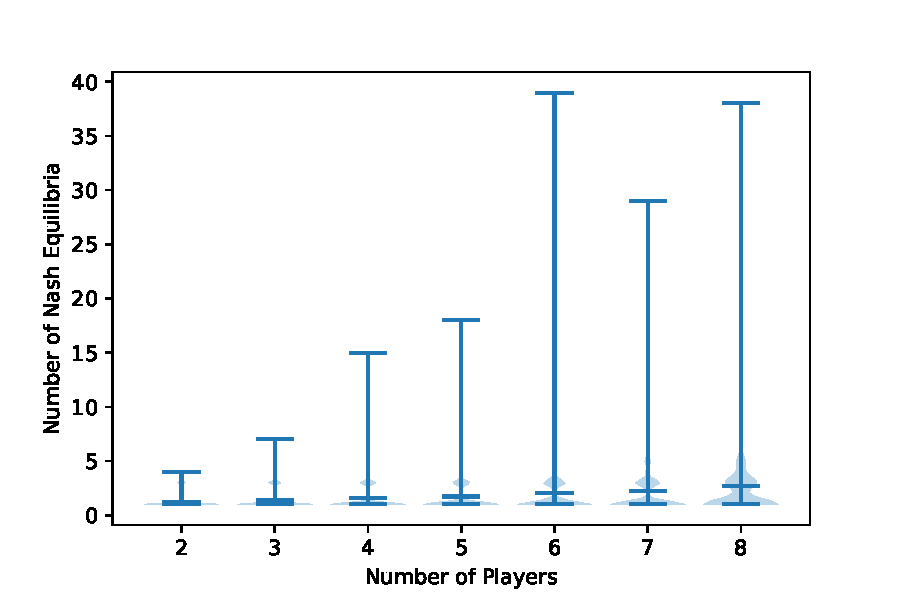
\includegraphics[width=\textwidth]{folk_thm/initial_analysis/player_num_of_equilibria_violinplot.pdf}
    \caption{A violinplot showing the distribution of the number of equilibria obtained for varying numbers of players.}\label{fig:NE_violinplot}
\end{figure}



\section{Analysis of the p-Threshold}\label{sec:Analysis_of_the_p-Threshold}

Firstly, for clarity, here is a restatement of the definition of a
\textit{\(p\)-threshold}: The value of \(p_{e}\) for which the
least probability of defection in Nash equilibria becomes zero.

In order to analyse the \(p\)-thresholds of the tournaments, a csv file was
created~\footnote{Please see the GitHub Repository
(https://github.com/shapperzsm/final-project)for the code used to obtain this
file. The csv file has also been archived at ().}
containing the
minimum, mean, median and maximum \(p\)-threshold probabilities for each
tournament set.
This was in order to gain as much information as possible from tournaments which
gave graphs such as in~\autoref{subfig:unclear_thresh_plot} described above. 
Within this file, other than the varying thresholds, the
information about the number of players, tournament set and \(p_{n}\) were
retained. Moreover, it contains a column which identifies whether any
of the strategy sets led to possible degenerate games.

An exploration into the overall \(p\)-thresholds is now given.

\begin{figure}
    \begin{subfigure}{0.45\textwidth}
        \centering
        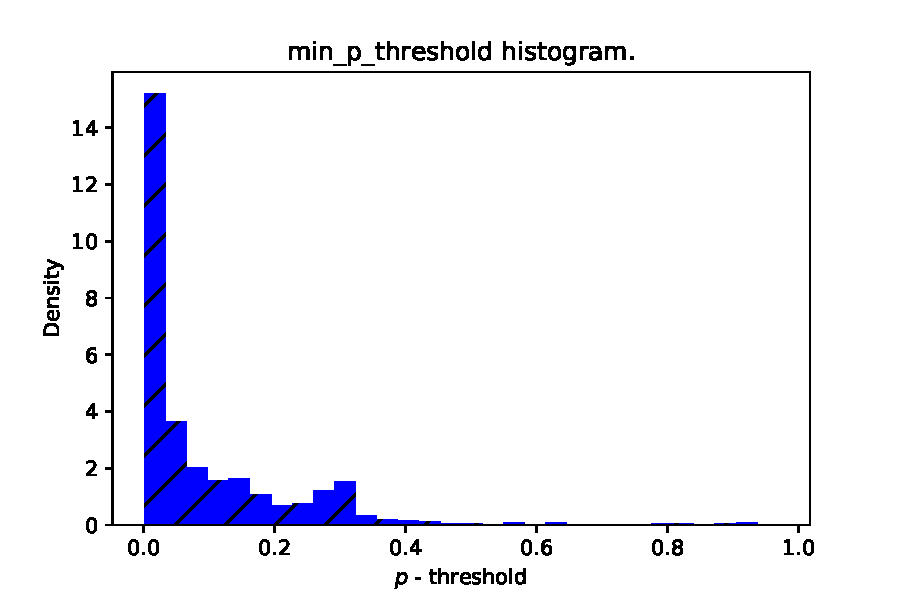
\includegraphics[width=\textwidth]{folk_thm/main_analysis/min_p_threshold_hist.pdf}
        \caption{A plot to show the minimum \(p\)-thresholds.}\label{subfig:min_p_thresh}
    \end{subfigure}
    \begin{subfigure}{0.45\textwidth}
        \centering
        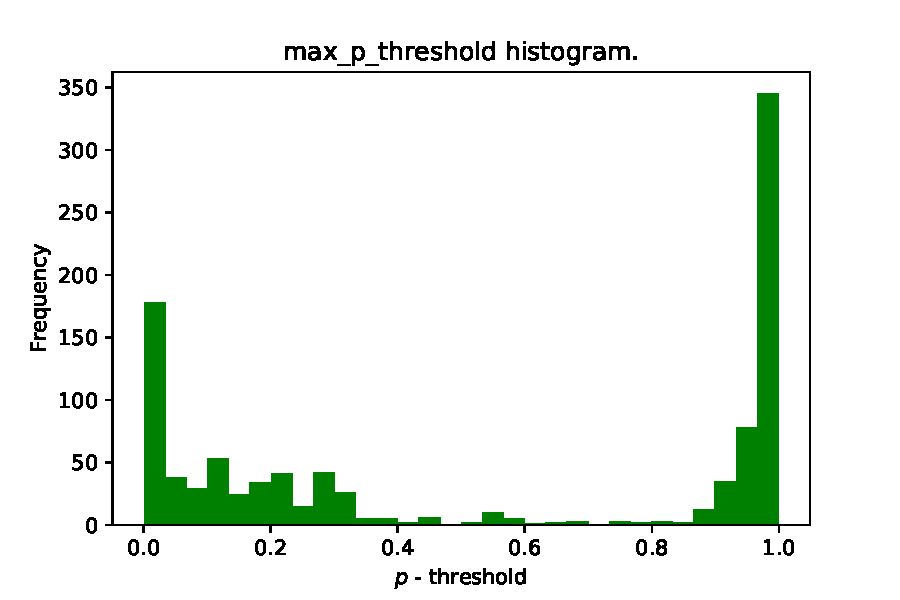
\includegraphics[width=\textwidth]{folk_thm/main_analysis/max_p_threshold_hist.pdf}
        \caption{A plot to show the maximum \(p\)-thresholds.}\label{subfig:max_p_thresh}
    \end{subfigure}
    \caption{Plots to show the \(p\)-thresholds for all 1001 sets of tournaments.}\label{fig:min_max_p_thresh}
\end{figure}

Observe, in~\autoref{subfig:min_p_thresh}, the majority of minimum \(p\)-thresholds
were less than 0.4, with a clear modal value of zero. That is, in a significant
proportion of the tournaments, there was no \(p_{e}\)
identified for
which the probability of defection was zero. Now considering~\autoref{subfig:max_p_thresh}, it can be seen that the modal value for the
maximum \(p\)-threshold is one.
Also, in comparison with the minimum \(p\)-threshold, there is a larger spread in the
density. Yet, there is still a peak around zero as with the minimum \(p\)-threshold
data. 

\begin{figure}
    \begin{subfigure}{0.45\textwidth}
        \centering
        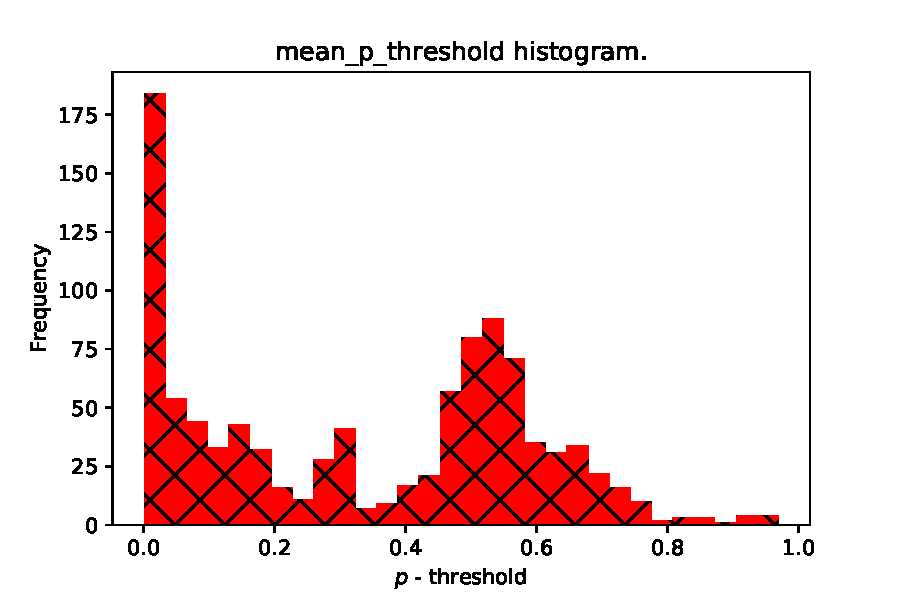
\includegraphics[width=\textwidth]{folk_thm/main_analysis/mean_p_threshold_hist.pdf}
        \caption{A plot to show the mean \(p\)-thresholds.}\label{subfig:mean_p_thresh}
    \end{subfigure}
    \begin{subfigure}{0.45\textwidth}
        \centering
        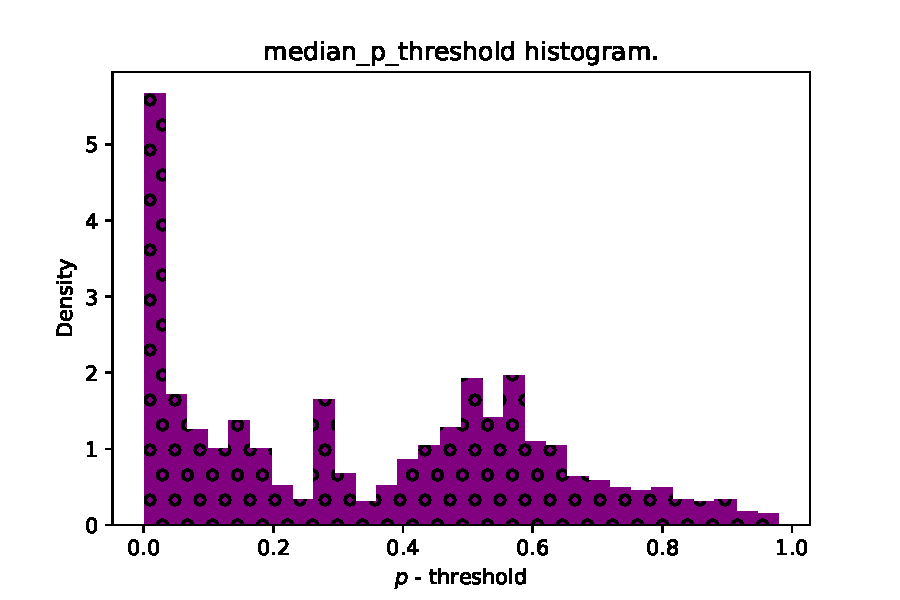
\includegraphics[width=\textwidth]{folk_thm/main_analysis/median_p_threshold_hist.pdf}
        \caption{A plot to show the median \(p\)-thresholds.}\label{subfig:median_p_thresh}
    \end{subfigure}
    \caption{Plots to show the \(p\)-thresholds for all 1001 sets of tournaments.}\label{fig:mean_median_p_thresh}
\end{figure}


Looking at the mean and median \(p\)-threshold data,~\autoref{fig:mean_median_p_thresh}, observe that the distributions obtained
are similar with, again, a modal value of zero, indicating that, for many games,
\(p_{e}\) has to be almost zero before defection becomes irrational. That is,
the probability of the game continuing is high. However, in
these histograms there is also a clear peak around a \(p\)-threshold of 0.5. This
suggests that some of the tournaments may have several \(p\)-thresholds, perhaps due
to stochasticity, degeneracy or just numerical experiment noise that appears in the 
tournaments. Indeed, obtaining the minimum and maximum
\(p\)-thresholds for those tournaments where the mean \(p\)-threshold was within the range
\([0.5, 0.6]\), it can be seen that, from~\autoref{fig:p_mean_middle_plot}
for a significant proportion, their minimum
threshold was around zero and their maximum around one. Moreover, looking closer
at three of the tournaments which satisfied the above, there is clear noise within the corresponding graphs,~\autoref{fig:p_mean_middle_specific}.


\begin{figure}
    \centering
    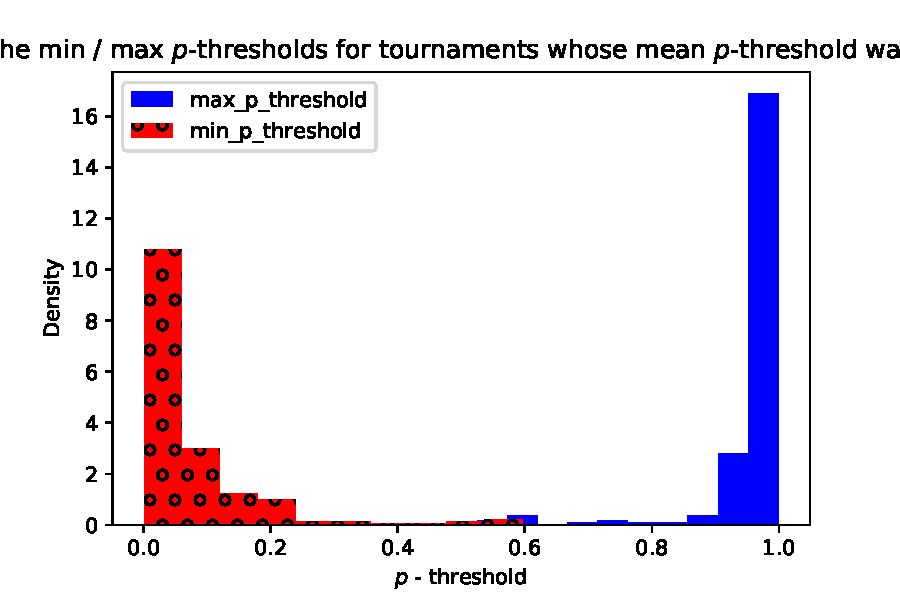
\includegraphics[width=\textwidth]{folk_thm/main_analysis/p_mean_middle_data_plot.pdf}
    \caption{A plot to show the minimum and maximum \(p\)-thresholds for those tournaments which had an mean threshold within the range \([0.5, 0.6]\).}\label{fig:p_mean_middle_plot}
\end{figure}


\begin{figure}
    \begin{subfigure}{0.3\textwidth}
        \centering
        \includegraphics[width=\textwidth]{folk_thm/single_game/6/105/0.2/main.pdf}
        \caption{6-player tournament set with \(p_{n}=0.2\), two stochastic players and no degeneracy was identified.}
    \end{subfigure}
    \begin{subfigure}{0.3\textwidth}
        \centering
        \includegraphics[width=\textwidth]{folk_thm/single_game/3/35/0.1/main.pdf}
        \caption{3-player tournament set with \(p_{n}=0.1\), one stochastic player and no degeneracy was identified.}
    \end{subfigure}
    \begin{subfigure}{0.3\textwidth}
        \centering
        \includegraphics[width=\textwidth]{folk_thm/single_game/3/33/0.5/main.pdf}
        \caption{3-player tournament set with \(p_{n}=0.5\), one stochastic player and only one tournament identified as degenerate, with \(p_{e}=0.9788\)}
    \end{subfigure}
    \caption{Example plots of the tournaments where the mean \(p\)-threshold was within the range \([0.5, 0.6]\).}\label{fig:mean_middle_specific}
\end{figure}

The plots contained in~\autoref{fig:mean_middle_specific} were sampled using the random library in Python. What is interesting here is that
they all contain varying amounts of standard PD noise and further analysis into
this would be beneficial. This could yield whether this is one of the main causes for the
inaccuracy of the thresholds. For example, looking at how many of the
tournaments with this property had \(p_{n} > 0\).

Regarding degeneracy, out of all 1754 tournaments, 372 were identified as
potentially leading to degenerate games.
These are omitted from the following plots in an attempt to focus on
non-degenerate games.

\begin{figure}
    \begin{subfigure}{0.45\textwidth}
        \centering
        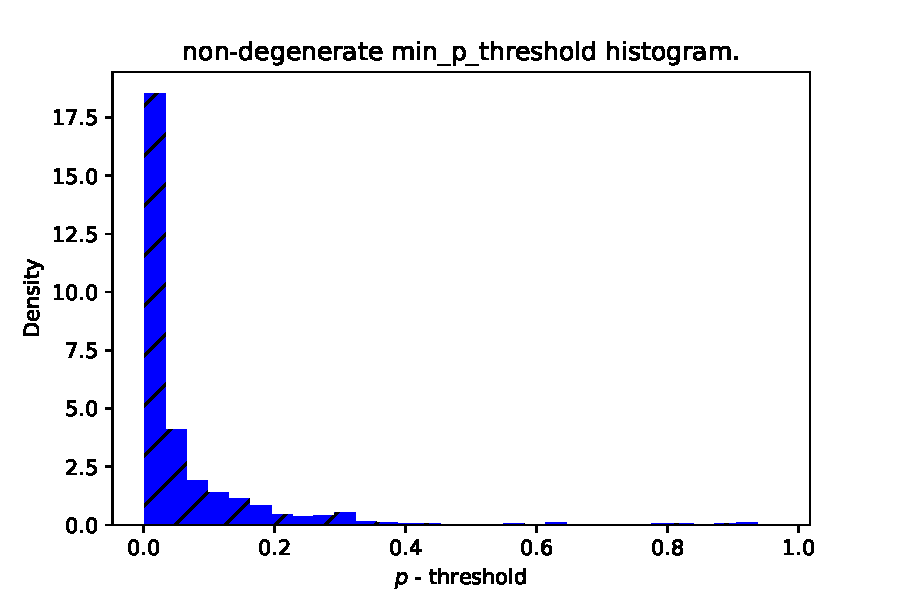
\includegraphics[width=\textwidth]{folk_thm/main_analysis/non-degen_min_p_threshold_hist.pdf}
        \caption{A plot to show the minimum \(p\)-thresholds.}\label{subfig:non_degen_min_p_thresh}
    \end{subfigure}
    \begin{subfigure}{0.45\textwidth}
        \centering
        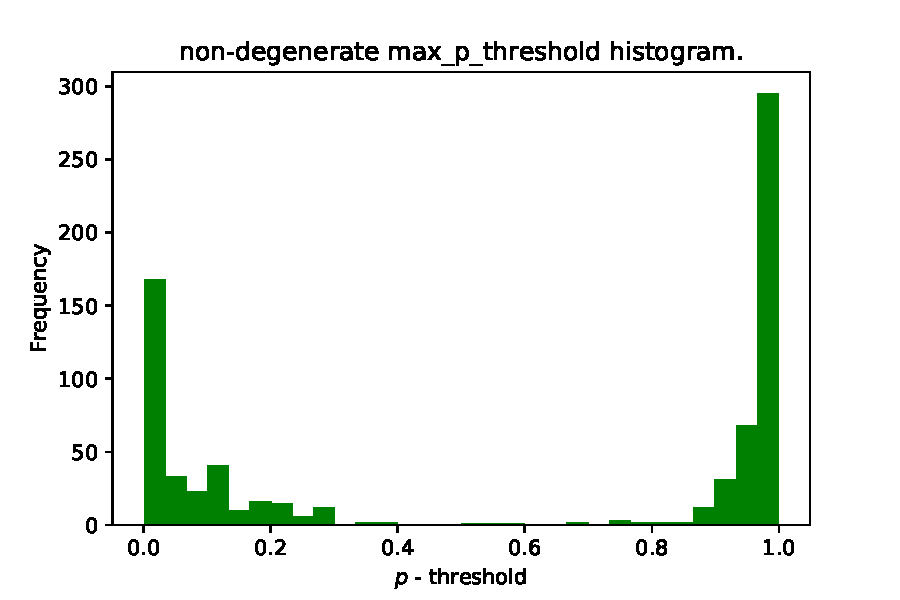
\includegraphics[width=\textwidth]{folk_thm/main_analysis/non-degen_max_p_threshold_hist.pdf}
        \caption{A plot to show the maximum \(p\)-thresholds.}\label{subfig:non_degen_max_p_thresh}
    \end{subfigure}
    \caption{Plots to show the \(p\)-thresholds for all tournaments which were not identified as degenerate.}\label{fig:non_degen_min_max_p_thresh}
\end{figure}


\begin{figure}
    \begin{subfigure}{0.45\textwidth}
        \centering
        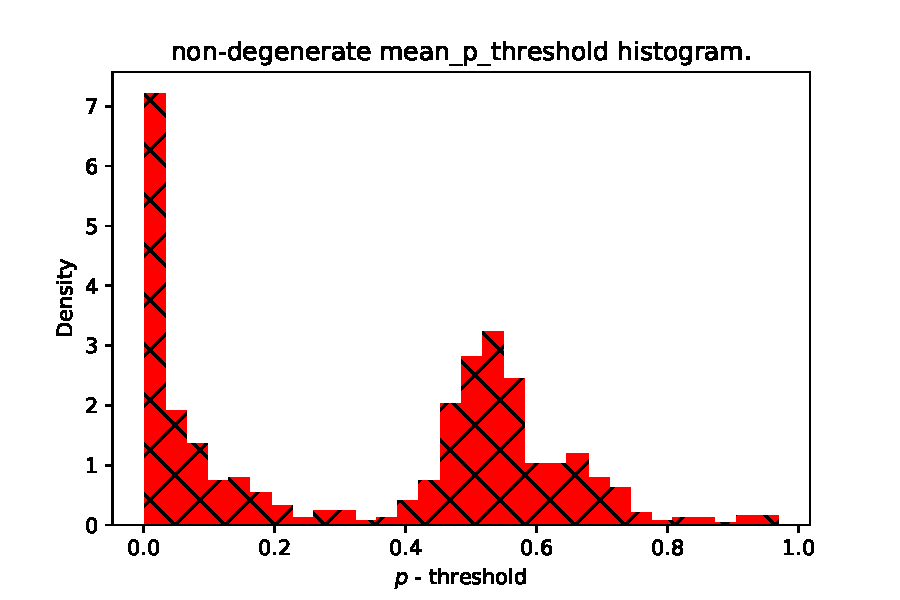
\includegraphics[width=\textwidth]{folk_thm/main_analysis/non-degen_mean_p_threshold_hist.pdf}
        \caption{A plot to show the mean \(p\)-thresholds.}\label{subfig:non_degen_mean_p_thresh}
    \end{subfigure}
    \begin{subfigure}{0.45\textwidth}
        \centering
        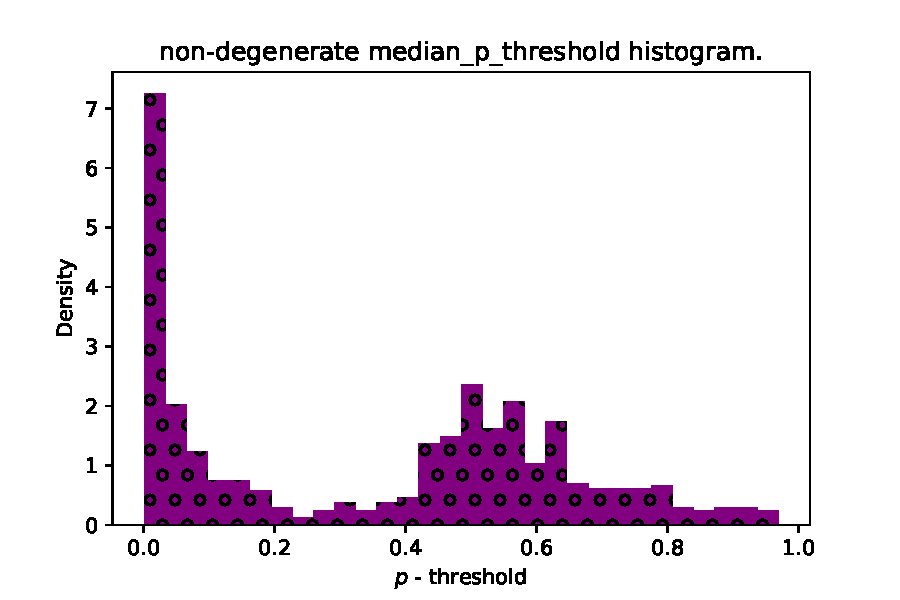
\includegraphics[width=\textwidth]{folk_thm/main_analysis/non-degen_median_p_threshold_hist.pdf}
        \caption{A plot to show the median \(p\)-thresholds.}\label{subfig:non_degen_median_p_thresh}
    \end{subfigure}
    \caption{Plots to show the \(p\)-thresholds for all tournaments which led to games not identified as degenerate.}\label{fig:non_degen_mean_median_p_thresh}
\end{figure}

Comparing~\autoref{subfig:non_degen_min_p_thresh},~\autoref{subfig:non_degen_max_p_thresh},~\autoref{subfig:non_degen_mean_p_thresh}
and~\autoref{subfig:non_degen_median_p_thresh} with~\autoref{subfig:min_p_thresh},~\autoref{subfig:max_p_thresh},~\autoref{subfig:mean_p_thresh}
and~\autoref{subfig:median_p_thresh}, respectively, it can be seen that, in general,
there is no significant change in the distributions of the thresholds. However,
there is a more prominent peak in~\autoref{subfig:mean_p_thresh} around 0.3
than in the corresponding potentially non-degenerate plot of~\autoref{subfig:non_degen_mean_p_thresh}. Further work regarding the effects
of degeneracy is advised as the identification of games which are degenerate is non-trivial.

\subsection{Effects of the Number of Players}\label{subsec:Effects_of_the_number_of_Players}
In this section, the \(p\)-thresholds will be analysed with respect to the
number of opponents the \textit{Defector} played against. Note, in this section,
any games identified as degenerate are omitted.


\begin{figure}
    \begin{subfigure}{0.45\textwidth}
        \centering
        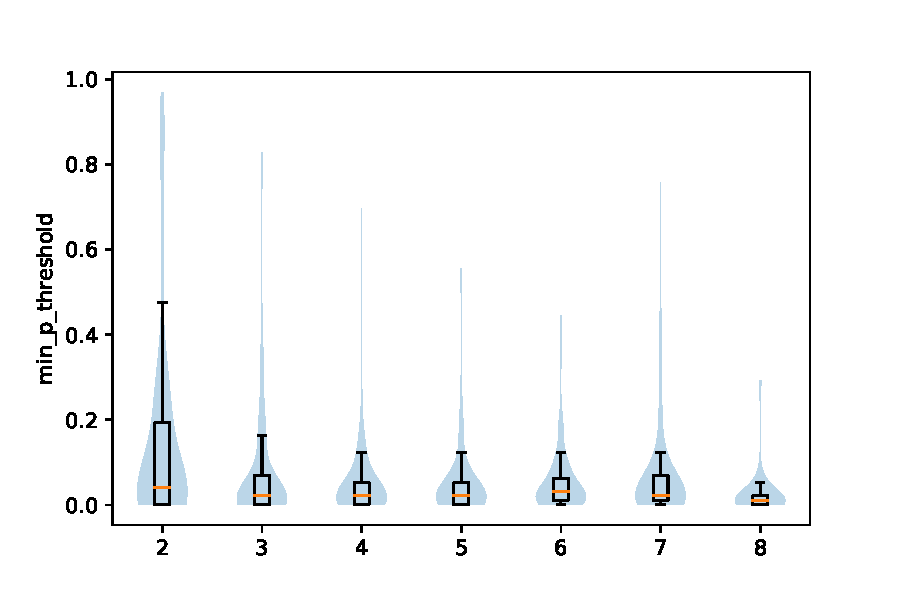
\includegraphics[width=\textwidth]{folk_thm/main_analysis/min_p_threshold_player_violinplot.pdf}
        \caption{Minimum \(p\)-threshold violinplot.}\label{subfig:min_thresh_player_violinplot}
    \end{subfigure}
    \begin{subfigure}{0.45\textwidth}
        \centering
        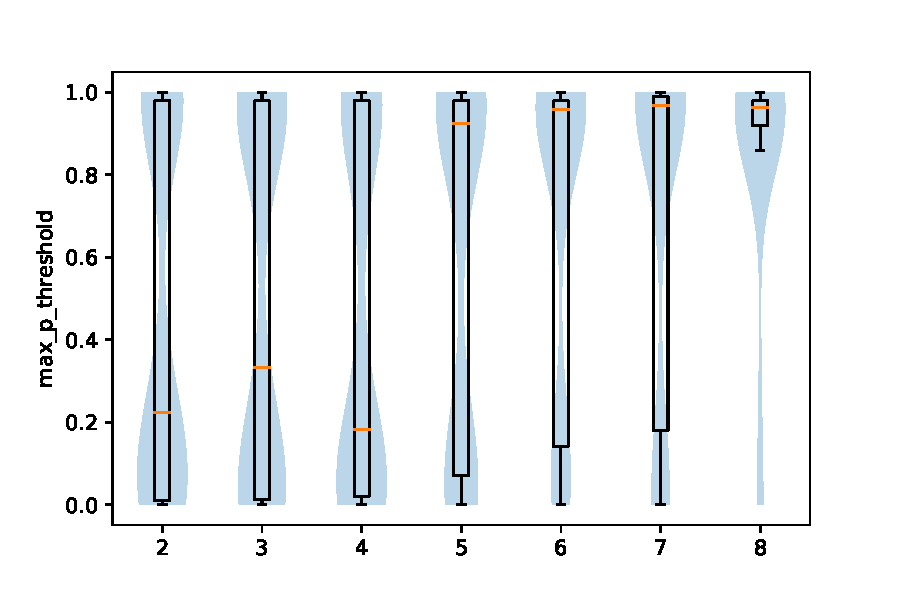
\includegraphics[width=\textwidth]{folk_thm/main_analysis/max_p_threshold_player_violinplot.pdf}
        \caption{Maximum \(p\)-threshold violinplot.}\label{subfig:max_thresh_player_violinplot}
    \end{subfigure}

    \begin{subfigure}{0.45\textwidth}
        \centering
        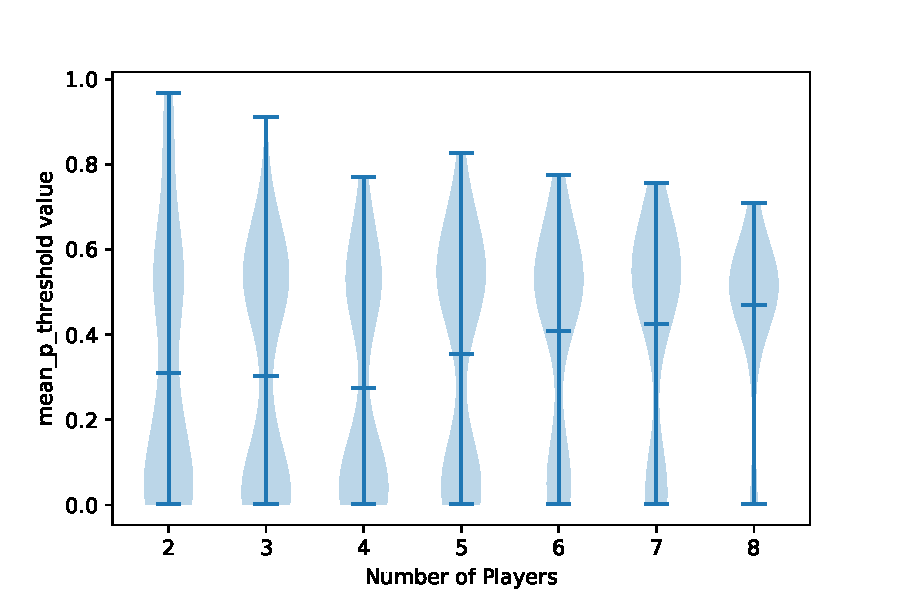
\includegraphics[width=\textwidth]{folk_thm/main_analysis/mean_p_threshold_player_violinplot.pdf}
        \caption{Mean \(p\)-threshold violinplot.}\label{subfig:mean_thresh_player_violinplot}        
    \end{subfigure}
    \begin{subfigure}{0.45\textwidth}
        \centering
        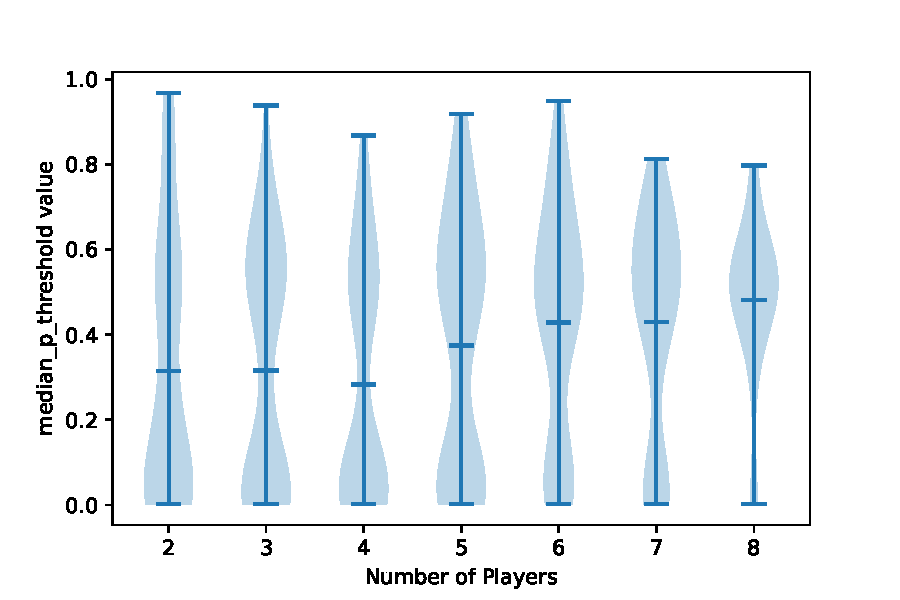
\includegraphics[width=\textwidth]{folk_thm/main_analysis/median_p_threshold_player_violinplot.pdf}
        \caption{Median \(p\)-threshold violinplot.}\label{subfig:median_thresh_player_violinplot}
    \end{subfigure}
    \caption{Violinplots of the thresholds for each number of opponents.}\label{fig:player_mean_thresh_violinplot}
\end{figure}

From~\autoref{subfig:min_thresh_player_violinplot}, it can be seen that the
distributions of the minimum \(p\)-thresholds, with respect to the number of
players, all have a modal value around zero. However, apart from the seven-player
tournaments, the spread of the distributions decrease, along with the mean
values. Considering the maximum \(p\)-thresholds,~\autoref{subfig:max_p_threshold_violinplot}, the distributions become bimodal
with mode values around zero and one. Yet, as the number of players increases the
modal value at zero becomes less prominent with the eight-player tournament
distribution not appearing to have a mode at zero. The variance of the distributions is
similar and, apart from four-player tournaments, the means increase with the number
of players. Looking now to the mean and median violinplots,~\autoref{subfig:mean_thresh_player_violinplot}
and~\autoref{subfig:median_thresh_player_violinplot} respectively, there is no
significant difference between the two plots, other than the spread is a little
larger in the median thresholds. Within the mean plot,~\autoref{subfig:mean_thresh_player_violinplot}, it can be seen that the
distributions also start off bimodal, with modal values at zero and approximately 0.5. However again, the
mode at zero becomes less distinct, with the eight-player tournament
distribution being unimodal. The modal value at around 0.5 is a consequence of
the reason stated previously. Moreover, observe that, apart from
four-player tournaments, the variance of the distributions seem to decrease with
the size of the player set whilst the means increase. These take a value of
approximately 0.3 for two-player tournaments to around 0.5 for eight-players. Looking
at~\autoref{fig:player_mean_thresh_violinplot} as a whole, it is implied
that the number of players has no significant effect on the value of the
\(p\)-threshold.


\subsection{Effects of Noise}\label{subsec:Effects_of_Noise}
Here, an analysis on the affect values of \(p_{n}\) have on the \(p\)-threshold is provided.
According to~\cite{glynatsi2020meta}, the addition of noise to a tournament indicates that, with a certain
probability, the action of a particular strategy is
altered. That is, an action of \(C\) changes to \(D\) and vice versa.  


\begin{figure}
    \begin{subfigure}{0.45\textwidth}
        \centering
        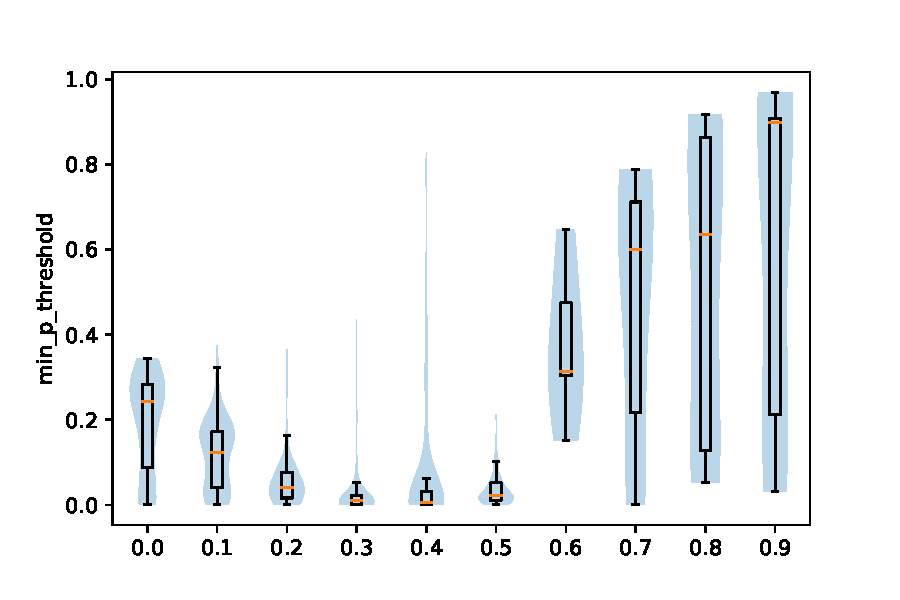
\includegraphics[width=\textwidth]{folk_thm/main_analysis/min_p_threshold_noise_violinplot.pdf}
        \caption{Minimum \(p\)-threshold violinplot.}\label{subfig:min_thresh_noise_violinplot}
    \end{subfigure}
    \begin{subfigure}{0.45\textwidth}
        \centering
        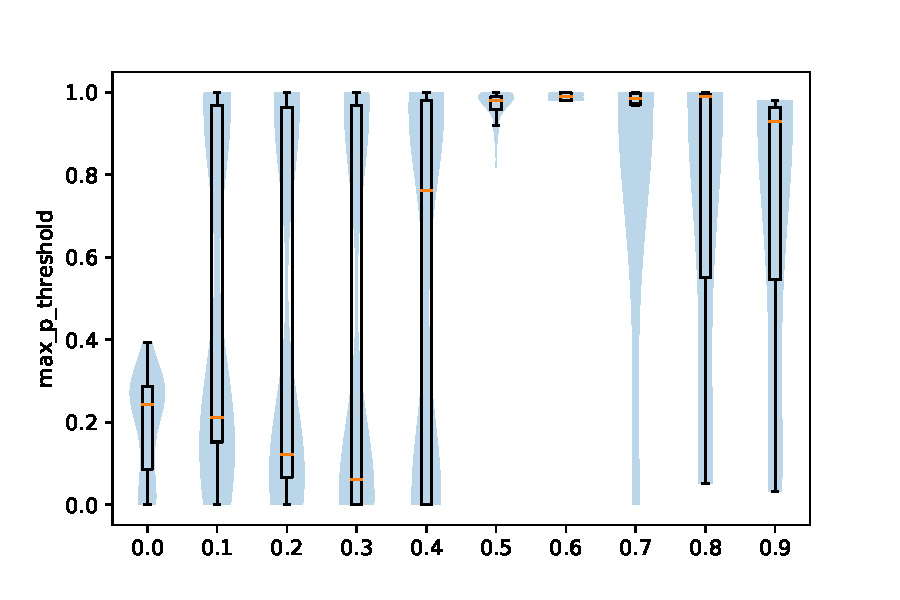
\includegraphics[width=\textwidth]{folk_thm/main_analysis/max_p_threshold_noise_violinplot.pdf}
        \caption{Maximum \(p\)-threshold violinplot.}\label{subfig:max_thresh_noise_violinplot}
    \end{subfigure}

    \begin{subfigure}{0.45\textwidth}
        \centering
        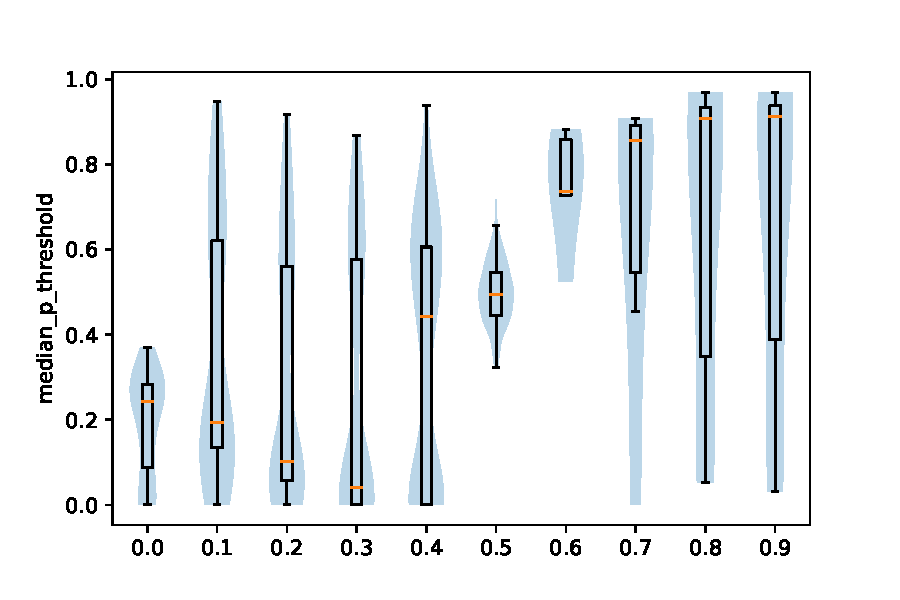
\includegraphics[width=\textwidth]{folk_thm/main_analysis/median_p_threshold_noise_violinplot.pdf}
        \caption{Median \(p\)-threshold violinplot.}\label{subfig:median_thresh_noise_violinplot}
    \end{subfigure}
    \begin{subfigure}{0.45\textwidth}
        \centering
        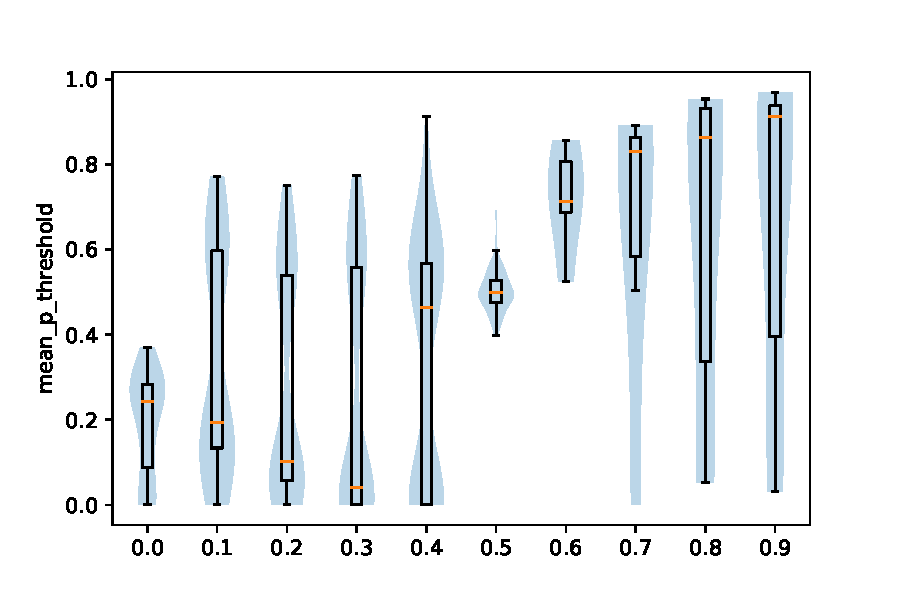
\includegraphics[width=\textwidth]{folk_thm/main_analysis/mean_p_threshold_noise_violinplot.pdf}
        \caption{Mean \(p\)-threshold violinplot.}\label{subfig:mean_thresh_noise_violinplot}
    \end{subfigure}
    \caption{Violinplots of the thresholds for each value of \(p_{n}\).}\label{fig:noise_p_thresh_violinplot}
\end{figure}

\autoref{subfig:min_thresh_noise_violinplot}, shows the distribution of the
minimum p-thresholds for each \(p_{n}\) value used in the
tournaments. It can be noted that the distributions of \(p_{n}\) values at
least 0.6 have a large variance, indicating that using a large value of
\(p_{n}\) is highly random and thus no conclusions can be drawn. On the
other hand, considering the noise levels less than 0.6, observe that the mean
\(p\)-thresholds decrease from around 0.25 to approximately zero as the noise
increases. These distributions are also clearly unimodal. Looking now at~\autoref{subfig:max_thresh_noise_violinplot}, it can be seen that the
majority of distributions have a much larger spread here varying over the full
spectrum of game-ending probabilities and similar observations can be made from~\autoref{subfig:median_thresh_noise_violinplot}
and~\autoref{subfig:mean_thresh_noise_violinplot}. 

\autoref{fig:single_set_vary_noise} shows an example of the same player set
through a variety of\(p_{n}\) values. Indeed, here it can clearly be seen that
the amount of
noise does effect the \(p\)-threshold. However, this is to be expected since, by
definition, as t\(p_{n}\) increases, the \textit{Defector} will be observed
as similar to the \textit{Cooperator} when \(p_{n}=0\).

\begin{figure}
    \begin{subfigure}{0.3\textwidth}
        \centering
        \includegraphics[width=\textwidth]{folk_thm/single_game/6/103/0.0/main.pdf}
        \caption{\(p_{n}=0\)}
    \end{subfigure}
    \begin{subfigure}{0.3\textwidth}
        \centering
        \includegraphics[width=\textwidth]{folk_thm/single_game/6/103/0.1/main.pdf}
        \caption{\(p_{n}=0.1\)}
    \end{subfigure}
    \begin{subfigure}{0.3\textwidth}
        \centering
        \includegraphics[width=\textwidth]{folk_thm/single_game/6/103/0.2/main.pdf}
        \caption{\(p_{n}=0.2\)}
    \end{subfigure}

    \begin{subfigure}{0.2\textwidth}
        \centering
        \includegraphics[width=\textwidth]{folk_thm/single_game/6/103/0.3/main.pdf}
        \caption{\(p_{n}=0.3\)}
    \end{subfigure}
    \begin{subfigure}{0.2\textwidth}
        \centering
        \includegraphics[width=\textwidth]{folk_thm/single_game/6/103/0.4/main.pdf}
        \caption{\(p_{n}=0.4\)}
    \end{subfigure}
    \begin{subfigure}{0.2\textwidth}
        \centering
        \includegraphics[width=\textwidth]{folk_thm/single_game/6/103/0.5/main.pdf}
        \caption{\(p_{n}=0.5\)}
    \end{subfigure}
    \begin{subfigure}{0.2\textwidth}
        \centering
        \includegraphics[width=\textwidth]{folk_thm/single_game/6/103/0.6/main.pdf}
        \caption{\(p_{n} \ge 0.6\)}
    \end{subfigure}
    \caption{Observation of one 6-player tournament set through the varying
    values of \(p_{n}\). There was one stochastic player and 13 out of
    the 1100 tournaments played yielded potential degenerate games. The opponents here were: \textit{Getzler};
    \textit{Punisher}; \textit{Forgiver}; \textit{GrudgerAlternator}; and \textit{GraaskampKatzen}.}\label{fig:single_set_vary_noise}
\end{figure}


Therefore, on the whole, there
are not many significant conclusions that can be made here. This implies that
the addition of noise to an already random tournament obscures any possible
visions of the \(p\)-threshold, especially as \(p_{n}\) increases.


\section{Conclusions and Further Work}\label{sec:Conclusions_and_Further_Work}
In this section, the beginnings of an analysis into the p-thresholds was
discussed. The effects of the number of players and level of standard PD noise on
these \(p\)-thresholds were the main focus, with a brief discussion regarding the
degeneracy of games also given. This turned out to be a non-trivial task due to
the three sources of noise potentially affecting the tournaments (standard PD
noise, stochasticity of players and numerical experiment noise) as well as the
difficulty in identifying degeneracy. However a few points of interest were highlighted and these are
summarised here. 

Firstly, the potential degeneracy of games yielded by the tournaments, at first
glance appears to not create much effect. The histograms of the p-thresholds, when the
tournaments including potential degeneracy were omitted, did not have any
significant changes when compared to the original histograms of all tournaments.
However, this could be due to the inclusion of unidentified degenerate games in
the non-degenerate plots and thus further exploration is advised here. Regarding the number of players in
a tournament, it was initially thought that this would be a key factor in
the variability of the \(p\)-threshold. However, on obtaining the distributions of
the \(p\)-thresholds for player sets of size two
to eight, it was implied that the number of players does not have a significant
impact. Finally, the effect of different values of \(p_{n}\) on
the \(p\)-threshold was analysed. Here, it was observed that, as expected, the level
of additional noise did affect the \(p\)-threshold however there were no significant
trends appearing out of the randomness.

As stated above, this is only the very start of an analysis into the
\(p\)-thresholds described by the `original' Folk Theorem~\cite{Friedman1971} and the effects of the
varying environmental factors in tournaments of the IPD. Thus many
questions regarding this are still to be researched and a few recommendations
regarding further work are now summarised. Firstly, it was observed that there were a
significant proportion of tournaments for which the graph remained constant at
zero or one. That is, the \(p\)-threshold was not identified using the precision of
game-ending probabilities chosen and therefore must lie within the intervals (0,
0.001) or (0.999, 1), respectively. Hence, these tournament sets could be rerun
with a much finer precision, within the appropriate intervals, to highlight
exactly what is happening here. Also, an analysis into the characteristics of
the strategies involved, and the value of \(p_{n}\) included, in these
tournaments could provide a clearer insight into potential reasons.
Moreover, with regards to analysing the characteristics of players, it is
suggested that those player sets in which stochastic players were included
could be repeated with the stochastic players removed. This could help in revealing whether
the stochasticity of the player has any effect on the \(p\)-threshold. 

To check the reliability of the data collected, a second
experiment is recommended using a different algorithm for calculating the Nash
equilibria, for example vertex enumeration. This could be used in comparison
with the data already collected to identify whether the algorithms are producing
the same Nash equilibria or, more importantly, whether they identify the same
games as degenerate. Furthermore, it is suggested that this experiment be
executed with a larger number of tournaments repeats (greater than 500) to
observe whether this `smooths' the payoff matrices with greater success to
enable for a clearer visualisation of the \(p\)-thresholds. Finally, some
multivariate data analysis of the results, for example regression, could provide
some more insights into this topic.

Overall, this chapter has been successful in visualising the Folk Theorem using
the data collection setup as explained in~\autoref{ch:Methods} and using the plots
obtained as in~\autoref{subfig:clear_thresh_plot}.
